%% Based on a TeXnicCenter-Template by Tino Weinkauf.
%%%%%%%%%%%%%%%%%%%%%%%%%%%%%%%%%%%%%%%%%%%%%%%%%%%%%%%%%%%%%

%%%%%%%%%%%%%%%%%%%%%%%%%%%%%%%%%%%%%%%%%%%%%%%%%%%%%%%%%%%%%
%% HEADER
%%%%%%%%%%%%%%%%%%%%%%%%%%%%%%%%%%%%%%%%%%%%%%%%%%%%%%%%%%%%%
%\documentclass[onecolumn, 11pt, conference, compsocconf]{IEEEtran}
\documentclass[onecolumn, 12pt, article]{IEEEtran}
\usepackage{times,color,amsmath,amssymb,amsthm,comment,graphicx,cite,multirow}
%\documentclass[letterpaper,oneside,11pt]{letter}
% Alternative Options:
%	Paper Size: a4paper / a5paper / b5paper / letterpaper / legalpaper / executivepaper
% Duplex: oneside / twoside
% Base Font Size: 10pt / 11pt / 12pt


%% Language %%%%%%%%%%%%%%%%%%%%%%%%%%%%%%%%%%%%%%%%%%%%%%%%%
\usepackage[USenglish]{babel} %francais, polish, spanish, ...
\usepackage[T1]{fontenc}
\usepackage[ansinew]{inputenc}

\usepackage{lmodern} %Type1-font for non-english texts and characters
\usepackage{algorithm}
\usepackage{algpseudocode}
\usepackage{float}

%% Packages for Graphics & Figures %%%%%%%%%%%%%%%%%%%%%%%%%%
%\usepackage{graphicx} %%For loading graphic files
%\usepackage{subfig} %%Subfigures inside a figure
%\usepackage{tikz} %%Generate vector graphics from within LaTeX

%% Please note:
%% Images can be included using \includegraphics{filename}
%% resp. using the dialog in the Insert menu.
%% 
%% The mode "LaTeX => PDF" allows the following formats:
%%   .jpg  .png  .pdf  .mps
%% 
%% The modes "LaTeX => DVI", "LaTeX => PS" und "LaTeX => PS => PDF"
%% allow the following formats:
%%   .eps  .ps  .bmp  .pict  .pntg


%% Math Packages %%%%%%%%%%%%%%%%%%%%%%%%%%%%%%%%%%%%%%%%%%%%
\usepackage{amsmath}
\usepackage{amsthm}
\usepackage{amsfonts}
\usepackage{amssymb}
%\usepackage{array,MnSymbol}


%% Line Spacing %%%%%%%%%%%%%%%%%%%%%%%%%%%%%%%%%%%%%%%%%%%%%
\usepackage{setspace}
\singlespacing        %% 1-spacing (default)
%\onehalfspacing       %% 1,5-spacing
%\doublespacing        %% 2-spacing


%% Other Packages %%%%%%%%%%%%%%%%%%%%%%%%%%%%%%%%%%%%%%%%%%%
%\usepackage{a4wide} %%Smaller margins = more text per page.
\usepackage{fancyhdr} %%Fancy headings
\usepackage{listings}
\usepackage{capt-of}


%
% Theorem like environments
%
\newtheorem{problem}{Problem}%
%\numberwithin{problem}{section}
\newtheorem{theorem}{Theorem}%
\newtheorem{acknowledgment}{Acknowledgment}%
%\newtheorem{algorithm}{Algorithm}%
\newtheorem{assumption}{Assumption}%
\newtheorem{axiom}{Axiom}%
\newtheorem{case}{Case}%
\numberwithin{case}{problem}
\newtheorem{claim}{Claim}%
\newtheorem{conclusion}{Conclusion}
\newtheorem{condition}{Condition}
\numberwithin{condition}{problem}
\numberwithin{condition}{subsection}
\newtheorem{conjecture}{Conjecture}
\newtheorem{corollary}{Corollary}
\newtheorem{criterion}{Criterion}
\newtheorem{definition}{Definition}
\numberwithin{definition}{section}
\newtheorem{example}{Example}
\newtheorem{exercise}{Exercise}%
\newtheorem{lemma}{Lemma}%
\newtheorem{notation}{Notation}%
\theoremstyle{remark}
\newtheorem{question}{Question}%
\numberwithin{question}{problem}
\theoremstyle{plain}
\newtheorem{answer}{Answer}%
\numberwithin{answer}{problem}
\newtheorem{proposition}{Proposition}%
\newtheorem{remark}{Remark}%
\newtheorem{solution}{Solution}%
\numberwithin{solution}{section}
\newtheorem{summary}{Summary}%
\numberwithin{equation}{section}%
\newtheorem{option}{Option}



\raggedbottom
%%%%%%%%%%%%%%%%%%%%%%%%%%%%%%%%%%%%%%%%%%%%%%%%%%%%%%%%%%%%%
%% Remarks
%%%%%%%%%%%%%%%%%%%%%%%%%%%%%%%%%%%%%%%%%%%%%%%%%%%%%%%%%%%%%
%
% TODO:
% 1. Edit the used packages and their options (see above).
% 2. If you want, add a BibTeX-File to the project
%    (e.g., 'literature.bib').
% 3. Happy TeXing!
%
%%%%%%%%%%%%%%%%%%%%%%%%%%%%%%%%%%%%%%%%%%%%%%%%%%%%%%%%%%%%%

%%%%%%%%%%%%%%%%%%%%%%%%%%%%%%%%%%%%%%%%%%%%%%%%%%%%%%%%%%%%%
%% Options / Modifications
%%%%%%%%%%%%%%%%%%%%%%%%%%%%%%%%%%%%%%%%%%%%%%%%%%%%%%%%%%%%%

%\input{options} %You need a file 'options.tex' for this
%% ==> TeXnicCenter supplies some possible option files
%% ==> with its-templates (File | New from Template...).




%% BEGIN DOCUMENT
\begin{document}

%% Title Page
\title{Insertion Sort Analysis in Java}
\author{Preston Stosur-Bassett}
\date{February 2, 2015}
\maketitle

\pagestyle{fancy}
\fancyhead[R]{Insertion Sort Analysis in Java, page \thepage}
\fancyhead[L]{Preston Stosur-Bassett}

%% BEGIN ABSTRACT
\begin{abstract}
%% TODO: Write abstract
%% END ABSTRACT
\end{abstract}

%% BEGIN MOTIVATION
\section{Motivation}
In order to show how an algorithm might run on a given set of hardware, and how the algorithm will perform when given large amounts of data, algorithms are analysed. More specifically, insertion sort is analysed to determined what the run time might be for sorting large amounts of data on any modern computer.
%% END MOTIVATION

%% BEGIN BACKGROUND
\section{Background}
A sorting algorithm is used to sort data with a natural order. One such sorting algorithm is insertion sort, which sorts by iterating through a list of data, taking the current position and repositioning it into a more appropriate place in the list. How will this procedure perform when handling high volumes of data? How will it perform when executed on different machines? Because insertion sort is a more basic sorting algorithm, numerous papers and articles have been written answering these two questions.
%% END BACKGROUND

%% BEGIN PROCEDURE
\section{Procedure}
An insertion sort can be implemented in a multitude of languages using the pseudocode provided below.
\newline
\textbf{Insertion Sort Pre-Condition}: A is a non-empty array of data with a natural order.
\newline
\textbf{Insertion Sort Post-Condition}: A' is a permutation of A (containing all the same elements) in strictly non-decreasing order.
\begin{algorithm}
\caption {\textsc{Insertion-Sort}(A)}
\label{algo:insertionsort}
\begin{algorithmic}[1]
\Procedure{Insertion-Sort}{A}
\If{$A.length <= 1$}
\State{\Return{$A$}}
\EndIf
\State{$i = 2$}
\While{$i$ upto $A.length$}
	\State{$key = A[i]$}
	\State{$j = i - 1$}
	\While{$j$ downto $1$ and $key < A[j]$}
		\State{$A[j + 1] = A[j]$}
		\State{$j = j - 1$}
	\EndWhile
	\State{$A[j+1] = key$}
	\State{$i = i + 1$}
\EndWhile
\EndProcedure
\end{algorithmic}
\end{algorithm}
\newline
\textbf{Outer-Loop Invariant}: The subarray A'[1 ... i - 1] contains all the same elements as the subarray A[1 .. i - 1].
\newline 
\textbf{Outer-Loop Initialization}: The outer-loop invariant holds because A'[1 ... i - 1] and A[1 ... i - 1] both contain the same one element.
\newline
\textbf{Outer-Loop Maintenance}: The outer-loop invariant holds because A'[1 ... i - 1] and A[1 ... i - 1] both contain the same elements, although they maybe in different orders.
\newline
\textbf{Outer-Loop Termination}: When the outer-loop terminates, i = A.length, which implies that the entire array has been traversed and the guard has been negated. The negation of the guard implies that A'[1 ... i - 1] contains all the elements in A[1 ... i - 1].
\newline
\newline
\textbf{Inner-Loop Invariant}: A'[1 ... j] is sorted in strictly non-decreasing order.
\newline
\textbf{Inner-Loop Initialization}: Before the first iteration of the loop, j = 1, meaning the subarray A'[1 ... j] contains exactly one element, which is already sorted.
\newline
\textbf{Inner-Loop Maintenance}: At the beginning of each iteration of the loop the inner-loop invariants holds because j counts down from i and A'[j+1] is swapped with A'[j] only if A'[j+1] is less than A[j].
\newline
\textbf{Inner-Loop Termination}: The negation of the implies that j = A.length and A'[1 ... j] has been entirely traversed and sorted in strictly non-decreasing order which maintains the inner-loop invariant. 
\newline
\newline
\textbf{Conclusion}: The termination of both the inner and outer loops implies that the entire array has been traversed, A' is a permutation of A containing all the same elements in strictly non-decreasing order. This satisfies the post condition.
%% END PROCEDURE

%% BEGIN TESTING
\section{Testing}
\subsection{Testing Plan and Results}
All arrays used in testing are Java ArrayList<Integer> unless otherwise specified. All times are recorded in milliseconds using a stopwatch class borrowed from [NEED CITATION]. %% TODO: Add Citation %%
It is important to note that the stopwatch class used takes the elapsed real-time between the start of the insertion sort algorithm and the end of the insertion sort algorithm as opposed to taking the elapsed processor-time because these tests were run on a multi-core computer. 
In the table below A denotes Array. Times in the table below are given as averages out of 10 trials.
\newline
\captionof{table}{Test Results}
\begin{center}
\begin{tabular}{|l|l|l|l|}
\hline Tested Input & Expected Results & Actual Results & Time \\
\hline Empty A & Empty A & Empty A & 0.0003 \\
\hline A of 1000 Strings & Sorted A 1000 Strings & Sorted A 1000 Strings & 0.021 \\
\hline A 1 Element & Original A & Original A & 0.0003 \\
\hline A 10 Elements & Sorted A 10 Elements & Sorted A 10 Elements & 0.0005 \\
\hline A 100 Elements & Sorted A 100 Elements & Sorted A 100 Elements & 0.0021 \\
\hline A 1000 Elements & Sorted A 1000 Elements & Sorted A 1000 Elements & 0.019 \\
\hline A 10000 Elements & Sorted A 10000 Elements & Sorted A 10000 Elements & 0.129 \\
\hline A 100000 Elements & Sorted A 100000 Elements & Sorted A 100000 Elements & 6.4923 \\
\hline A 1000000 Elements & Sorted A 1000000 Elements & Sorted A 1000000 Elements & 2135.5007 \\
\hline A 10000000 Elements & Sorted A 10000000 Elements & OS Crash & N/A \\
\hline A 1000 Identical Elements & Original Array & Original Array & 0.0052 \\
\hline
\end{tabular}
\end{center}

\subsection{Problems Encountered}
One major issue encountered during the development of this insertion sort was that after completing the sort, A' was completely sorted properly except for the first element in the array. No matter what value the first element of A had, it did not change position in A'. For example, if A[5, 6, 3, 4, 7] was passed to the insertion sort algorithm, the returned array would look like A'[5, 3, 4, 6, 7]. Changing the guard for the inner for loop (see Algorithm 1 line 6) from \textit{key < A[j] and j downto 1} to \textit{j downto 1 and key < A[j]} corrected this issue.
%% END TESTING

%% BEGIN EXPERIMENTAL ANALYSIS
\section{Experimental Analysis}
 The insertion sort demonstrated in Algorithm 1 was implemented in Java and executed on an HP SprectreXT TouchSmart with 4 Core Intel i7 processor clocked at 1.9GHz running Ubuntu Gnome 14.10 64-bit.
 \begin{figure}[!]
\begin{center}
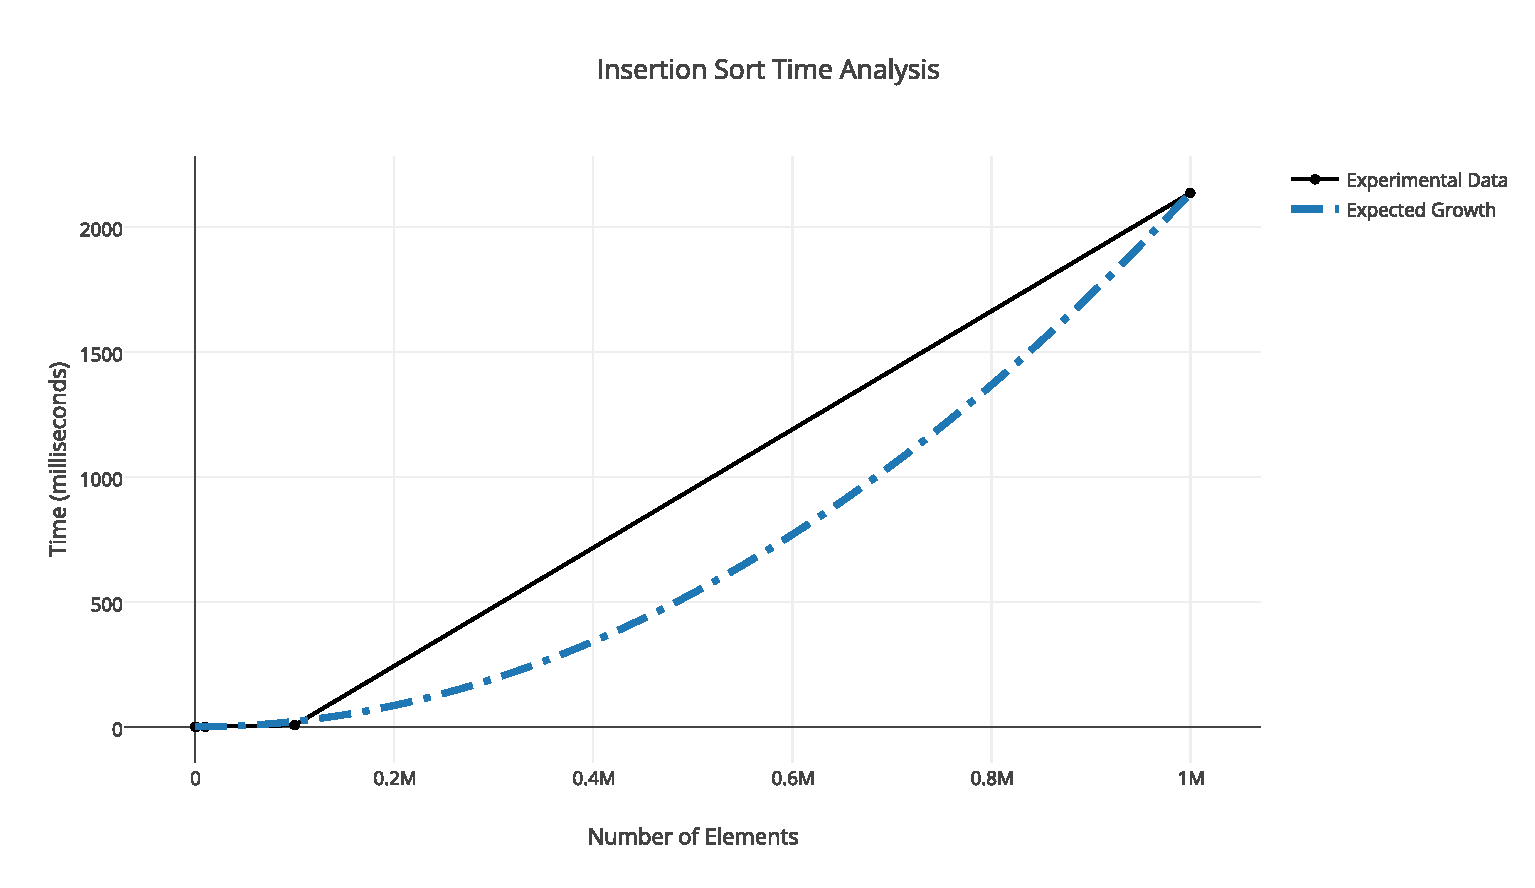
\includegraphics[scale=.75]{insertion_sort_time_analysis.pdf}
\end{center}
\captionof{figure}{Insertion Sort Time Analysis}
\label{fig:insertionsorttimeanalysis}
\end{figure}

The expected growth of insertion sort as the number of elements (n) grows large can be represented as $ \theta(n^2) $ where $ \theta() $ represents the asymptotically tightly bound running time. At $n_0$ the algorithm took 0.0003 milliseconds to complete. At $n_1$ the algorithm also took 0.0003 milliseconds to complete. For both these values of $n$, the algorithm runs at a constant time because no for-loops are executed. As $n$ grows larger the time to complete the experimental data correlates quite accurately with the expected growth. For $n_{1*10^6} $ the data matches up perfectly. This is to be expected however, because as n grows larger the constants and lower orders of the actual running time of the insertion sort start to effect the the running time less and less because the highest order of $n^2$ is so large. 
%% END EXPERIMENTAL ANALYSIS

%% BEGIN CONCLUSION
\section{Conclusions}

%% END CONCLUSION

\newpage

%% BEGIN REFERENCES
\section*{References}

%% END REFERENCES

\newpage

%% BEGIN APPENDIX
\section*{Appendix}
\lstinputlisting[caption=TestDriver,
label={TestDriver.java},
breaklines=true,
]{Code/TestDriver.java}
\lstinputlisting[caption=Debug,
label={Debug.java},
breaklines=true,
]{Code/Debug.java}
\lstinputlisting[caption=DummyData,
label={DummyData.java},
breaklines=true,
]{Code/DummyData.java}

The class Stopwatch has not been altered from its original form.
\newline
\lstinputlisting[caption=Stopwatch,
label={Stopwatch.java}
breaklines=true,
]{Code/Stopwatch.java}
\lstinputlisting[caption=Sort,
label={Sort.java},
breaklines=true,
]{Code/Sort.java}
%% END APPENDIX

%% END DOCUMENT
\end{document}
